\documentclass[b0paper,margin=1cm,landscape]{baposter}

\usepackage{lipsum}          % This is just for some blindtext

\usepackage{relsize}	       % For \smaller
\usepackage{url}			       % For \url
\usepackage{epstopdf}	       % Included EPS files automatically converted to PDF to include with pdflatex
\usepackage{multicol}        % Multi Columns

\usepackage{amsmath,amssymb} % math
\usepackage{natbib}
\usepackage{graphicx}
\usepackage{xcolor}
\usepackage{hyperref}

\definecolor{umblue}{rgb}{0.03, 0.15, 0.30}
\definecolor{ummaize}{rgb}{0.90, 0.85 0.40}

%%%%%%%%%%%%%%%%%%%%%%%%%%%%%%%%%%%%%%%%%%%%%%%%%%%%%%%%%%%%%%%%%%%%%%%%%%%%%%%%
%%% Utility functions %%%%%%%%%%%%%%%%%%%%%%%%%%%%%%%%%%%%%%%%%%%%%%%%%%%%%%%%%%
%%%%%%%%%%%%%%%%%%%%%%%%%%%%%%%%%%%%%%%%%%%%%%%%%%%%%%%%%%%%%%%%%%%%%%%%%%%%%%%%

%%% Save space in lists. Use this after the opening of the list %%%%%%%%%%%%%%%%
\renewcommand{\vec}[1]{\bm{#1}}
\newcommand{\vnabla}{\vec{\nabla}}

\renewcommand{\d}[1]{\text{d} #1}
\newcommand{\dxx}{\,\text{d}\vec{x}}
\newcommand{\dx}{\,\text{d}x}

\newcommand{\diff}[2]{\frac{\text{d}#1}{\text{d}#2}}
\newcommand{\idiff}[2]{\text{d}#1 / \text{d}#2}
\newcommand{\pdiff}[2]{\frac{\partial #1}{\partial #2}}
\newcommand{\pdifff}[2]{\frac{\partial^2 #1}{\partial #2^2}}
\newcommand{\ipdiff}[2]{\partial #1 / \partial #2}
\newcommand{\vdiff}[2]{\frac{\delta #1}{\delta #2}}
\newcommand{\ivdiff}[2]{\delta #1 / \delta #2}

%%%%%%%%%%%%%%%%%%%%%%%%%%%%%%%%%%%%%%%%%%%%%%%%%%%%%%%%%%%%%%%%%%%%%%%%%%%%%%%
%%% Document Start %%%%%%%%%%%%%%%%%%%%%%%%%%%%%%%%%%%%%%%%%%%%%%%%%%%%%%%%%%%%
%%%%%%%%%%%%%%%%%%%%%%%%%%%%%%%%%%%%%%%%%%%%%%%%%%%%%%%%%%%%%%%%%%%%%%%%%%%%%%%

\begin{document}
\typeout{Poster rendering started}

%%% General Poster Settings %%%%%%%%%%%%%%%%%%%%%%%%%%%%%%%%%%%%%%%%%%%%%%%%%%%
%%%%%% Eye Catcher, Title, Authors and University Images %%%%%%%%%%%%%%%%%%%%%%
\begin{poster}{
  columns=4,
	grid=false,
	borderColor=umblue,
	headerColorOne=umblue,
	headerColorTwo=umblue,
	headerFontColor=ummaize,
  headerheight=14em,
	boxColorOne=white,
  boxpadding=1em,
	headershape=rectangle,
	headerfont=\Large\textsf,
	textborder=none,
	background=shadetb,
  bgColorOne=white,
  bgColorTwo=white,
	headerborder=open,
  boxshade=plain,
  headershade=plain,
  eyecatcher=false
}
%%% Eye Catcher %%%%%%%%%%%%%%%%%%%%%%%%%%%%%%%%%%%%%%%%%%%%%%%%%%%%%%%%%%%%%%%
{
}
%%% Title %%%%%%%%%%%%%%%%%%%%%%%%%%%%%%%%%%%%%%%%%%%%%%%%%%%%%%%%%%%%%%%%%%%%%
{Assessing the Ecology of the Flint River, Above and Below a Century-Old Dam}
%%% Authors %%%%%%%%%%%%%%%%%%%%%%%%%%%%%%%%%%%%%%%%%%%%%%%%%%%%%%%%%%%%%%%%%%%
{
  \vspace{0mm}
  \text{Chloe Summers} : \textit{\color{violet}{summersj@umich.edu}}, 
  \text{Arianna Elkins} : \textit{\color{violet}{arelkins@umich.edu}}, 
  \text{Cason Konzer} : \textit{\color{violet}{casonk@umich.edu}}, 
  \text{Heather Dawson} : \textit{\color{violet}{hdawson@umich.edu}} 
  
  \hspace{1mm} $\downharpoonright$ website : \textit{\color{violet}{https://flintriverecostudy.com}}
  \hspace{1mm} $\downharpoonright$ repository : \textit{\color{violet}{https://github.com/casonk/Flint\_River\_Ecology}}

}
%%% Logo %%%%%%%%%%%%%%%%%%%%%%%%%%%%%%%%%%%%%%%%%%%%%%%%%%%%%%%%%%%%%%%%%%%%%%
{
  \begin{minipage}{8.0em}
    
\includegraphics[height=8em]{Img/Ecology_Study.png}
  \end{minipage}
  \begin{minipage}{8.0em}
    
\includegraphics[height=8em]{Img/University_of_Michigan_Flint.png}
  \end{minipage}
}

%%% Abstract %%%%%%%%%%%%%%%%%%%%%%%%%%%%%%%%%%%%%%%%%%%%%%%%%%%%%%%%%%%%%%%%%%
\headerbox{Abstract}{name=box00, column=0, row=0}{

  \hspace{5mm} 

  \hspace{5mm}

  \hspace{5mm}
}

%%% Abstract %%%%%%%%%%%%%%%%%%%%%%%%%%%%%%%%%%%%%%%%%%%%%%%%%%%%%%%%%%%%%%%%%%
\headerbox{Reference}{name=box01, column=0, row=1, above=bottom, below=box00}{

  \hspace{5mm} 

  \hspace{5mm} 

}

%%% Graphics %%%%%%%%%%%%%%%%%%%%%%%%%%%%%%%%%%%%%%%%%%%%%%%%%%%%%%%%%%%%%%%%%%
\headerbox{Figure}{name=box10, column=1, row=0}{

  \hspace{5mm}


}


%%% Descriptions %%%%%%%%%%%%%%%%%%%%%%%%%%%%%%%%%%%%%%%%%%%%%%%%%%%%%%%%%%%%%%%%%%%%%
\headerbox{Figure Descriptions}{name=box20, column=2, row=0}{

  \hspace{5mm}

  Simpson's Diversity Index 
  $ \displaystyle D = 1 - \frac {\sum n(n-1)} {N(N-1)} $

}

%%% Descriptions %%%%%%%%%%%%%%%%%%%%%%%%%%%%%%%%%%%%%%%%%%%%%%%%%%%%%%%%%%%%%%%%%%%%%
\headerbox{}{name=box30, column=3, row=0}{

  \hspace{5mm}
  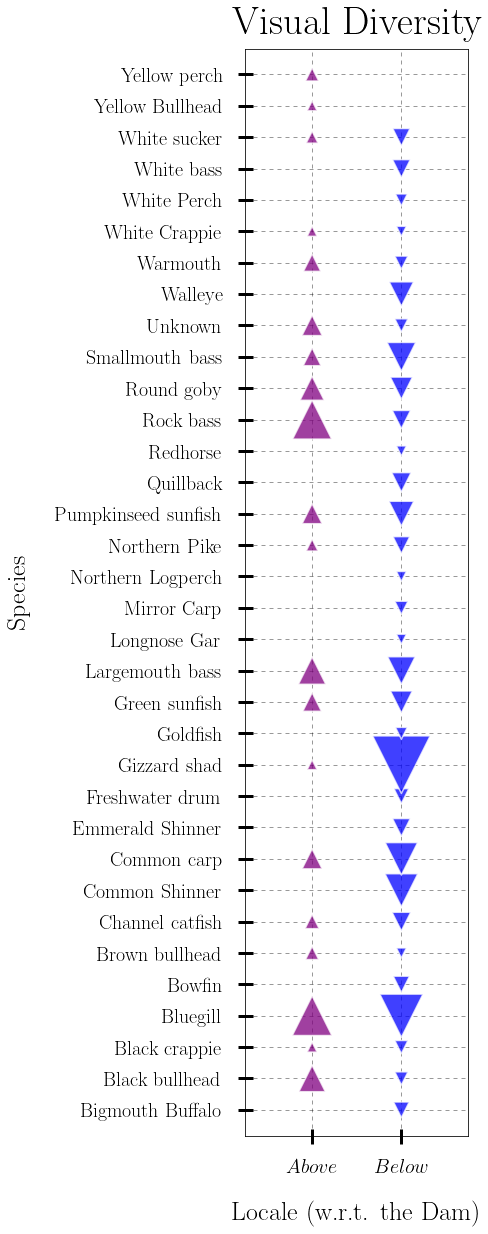
\includegraphics[width=.8\textwidth]{Img/Diversity_Bubble_Plot.png}

}

\end{poster}
\end{document}
